\section{Introduction}

embedded-ppc-g4-board is a full system simulator of an MPC7447A/MPC107 (PowerPC) based board. The simulated board is very similar to a PowerMac G4 PCI machine. Computations on IEEE 754 floating point numbers are emulated using simfloat. Altivec instructions are currently decoded but not implemented. The board is connected to its external environment through a PCI target which communicates with an external tool, either a co-simulation environment, an in-house industrial simulation environment, or even a testbench. Software running on the simulated hardware can be debugged by connecting a GDB client to the simulator through the GDB serial remote protocol. The GDB client can be either the standard text based client (i.e. command gdb), a graphical front-end to GDB (e.g. ddd), or even Eclipse CDT.

\begin{figure}[!h]
	\begin{center}
		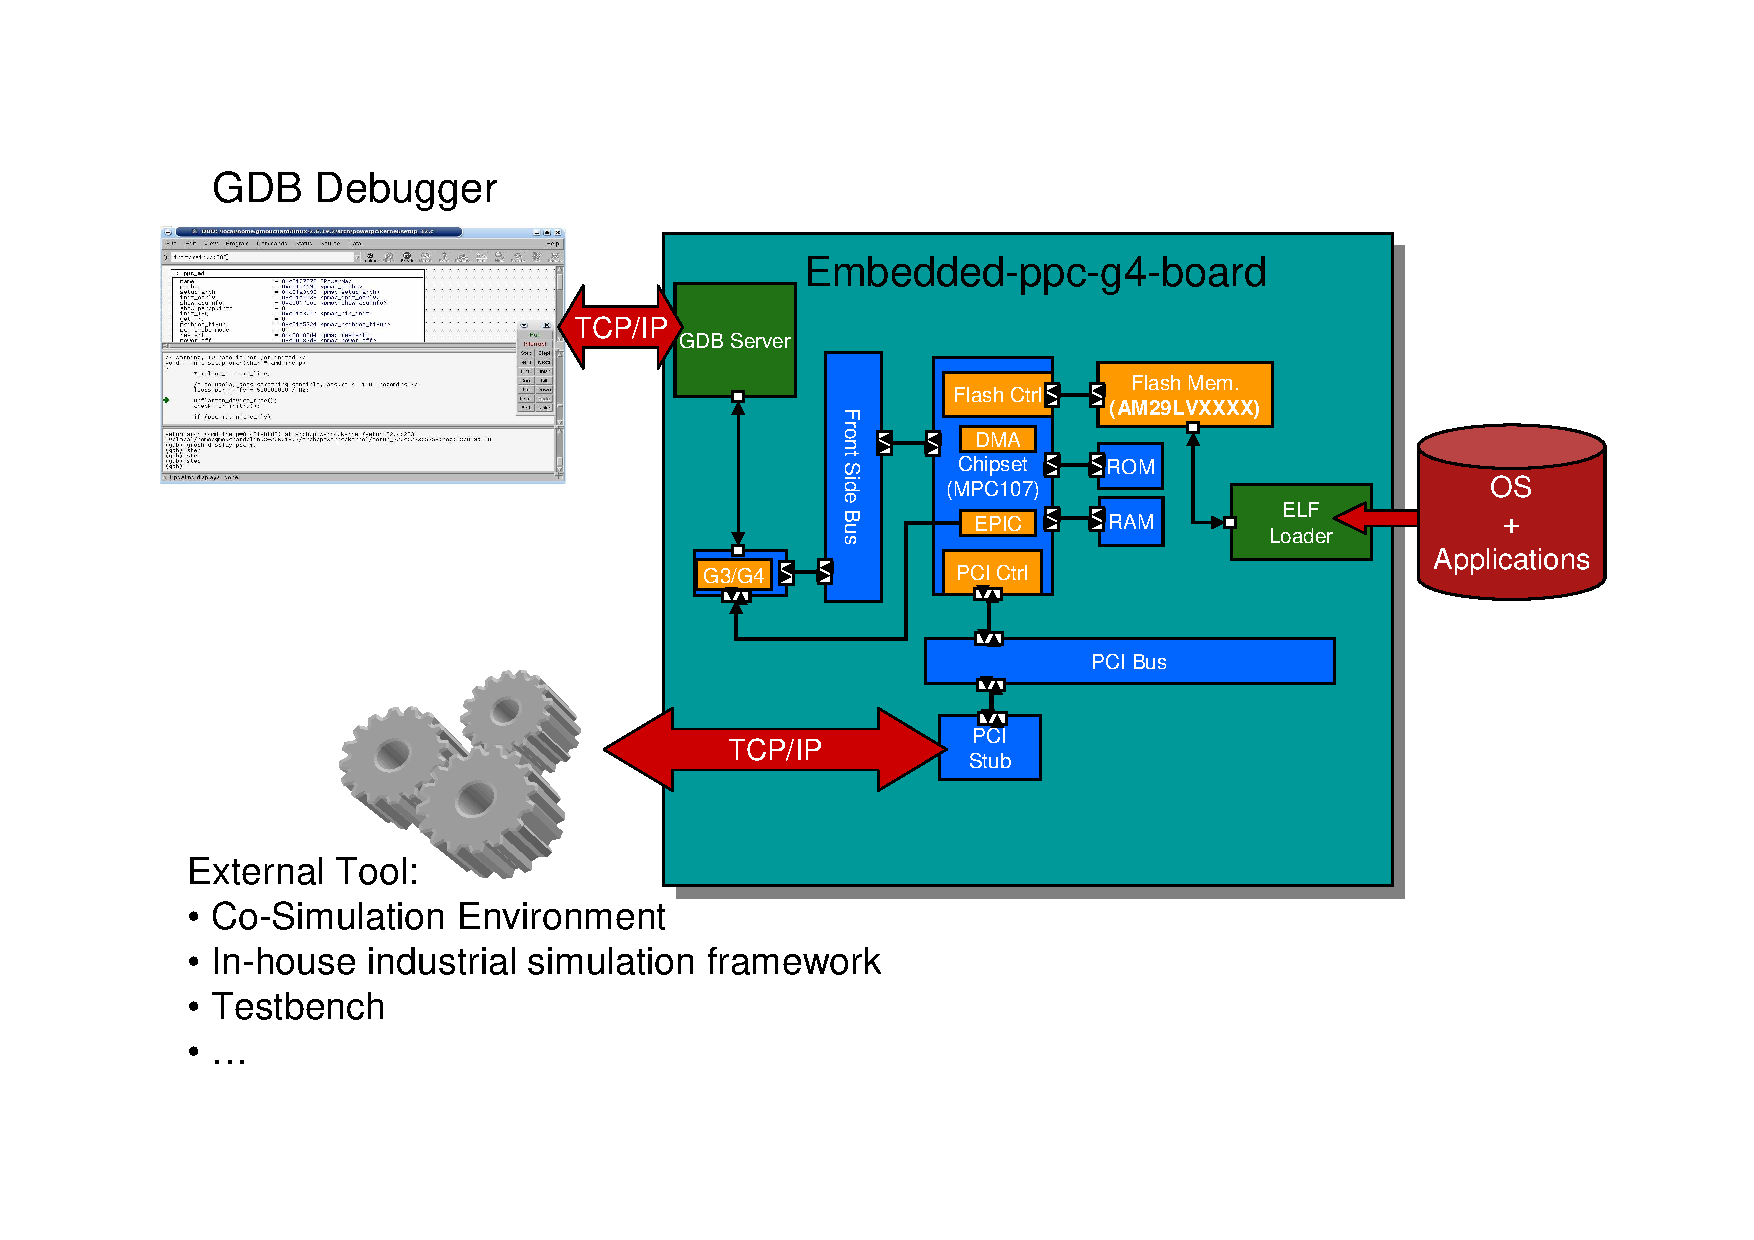
\includegraphics[width=\textwidth]{embedded_ppc_g4_board/fig_embedded_ppc_g4_board.pdf}
	\end{center}
	\caption{embedded-ppc-g4-boad simplified schematic.}
	\label{fig:ppcemu_system}
\end{figure}

\section{Simulated configuration}

The simulator is composed of the following modules:
\begin{itemize}\addtolength{\itemsep}{-0.40\baselineskip}
\item PowerPC CPU configured as an MPC7447A
\item snooping bus (front side bus)
\item MPC107 chipset
\item memory
\item rom
\item AM29LVxxx flash memory configured as an AM29LV800
\item PCI bus
\item PCI Stub
\end{itemize}

The simulator uses the following services:
\begin{itemize}\addtolength{\itemsep}{-0.40\baselineskip}
\item ELF Loader
\item GDB Server
\item Inline debugger
\item SystemC Time
\item Host Time
\item Power Estimators (for ITLB, DTLB, IL1, DL1 and L2)
\end{itemize}

\section{Using the simulator}

Usage: \texttt{embedded-ppc-g4-board [<options>] <firmware file1> [<firmware file2>...]}

Options:

\begin{itemize}

\item Starting the inline debugger

\texttt{--inline-debugger}
\texttt{-d}

\item Starting a GDB server

\texttt{--gdb-server <TCP port>}
\texttt{-g <TCP port>}

The GDB server will wait for a GDB client connection on the specified TCP port.

\item Defining the architecture description to be used by the GDB server

\texttt{--gdb-server-arch-file <arch file>}
\texttt{-a  <arch file>}

\item Defining the number of instructions to simulate before exiting

\texttt{-i <count>}
\texttt{--max:inst <count>}

\item Enabling power estimation for ITLB, DTLB, IL1, DL1, and L2

\texttt{-p}
\texttt{--power}

\item Redirecting the logger output into a file

\texttt{-l <file>}
\texttt{--logger:file <file>}

\item Enabling compression (gzip format) of the logger output

\texttt{-z}
\texttt{--logger:zip}

\item Redirecting the logger output to the standard error output

\texttt{-e}
\texttt{--logger:error}

\item Redirecting the logger output to the standard output

\texttt{-o}
\texttt{--logger:out}

\item Using file system pipes instead of TCP/IP for the pci-stub communications

\texttt{-u <pipe name>}
\texttt{--pci-stub-use-pipe <pipe name>}

\item Specifying the server name for pci-stub

\texttt{-s <server name>}
\texttt{--pci-stub-server <server name>}

\item Specifying the TCP port used by pci-stub

\texttt{-r <tcp port>}
\texttt{--pci-stub-tcp-port <tcp port>}

\item Making pci-stub act as a server instead of a client

\texttt{-v}
\texttt{--pci-stub-is-server}

\item Specifying the pci-stub regions (up to 6 separated by one or more space characters). ‘address space’ is either ‘mem’ or ‘i/o’

\texttt{-n <base address>,<byte size>,<address space>[...]}
\texttt{--pci-stub-regions <base address>,<byte size>,<address space>[...]}

\item Specifying the pci-stub IRQ number

\texttt{-q <irq number>}
\texttt{--pci-stub-irq <irq number>}

\item Forcing the ELF Loader to use segment virtual address instead of segment physical address

\texttt{-f}
\texttt{--force-use-virtual-address}

\item Specifying the ram memory size (default = 256MB)

\texttt{-b <ram memory size in MB>}
\texttt{--ram-size <ram memory size in MB>}

\item Displaying the integrated help

\texttt{--help}
\texttt{-h}

\end{itemize}